\documentclass[letterpaper]{article}
\usepackage{graphicx}

\begin{document}

\title{ECE 350: Digital Systems Project Checkpoint 4 Technical Report}
\author{Natalia Androsz}
\date{October 30, 2018}
\maketitle

\section*{Duke Community Standard}

By submitting this \LaTeX{} document, I affirm that
\begin{enumerate}
    \item I understand that each \texttt{git} commit I create in this repository is a submission
    \item I affirm that each submission complies with the Duke Community Standard and the guidelines set forth for this assignment
    \item I further acknowledge that any content not included in this commit under the version control system cannot be considered as a part of my submission.
    \item Finally, I understand that a submission is considered submitted when it has been pushed to the server.
\end{enumerate}

\section{Introduction}
This technical report described the design of a five-stage, single-issue, 32-bit processor in structural Verilog. The processor operates with a 50MHz clock and is to be deployed on an FPGA. The design integrates previously constructed processor elements -- a register file, an ALU, and multdiv. The pipeline "latches" to store data as instructions move from stage to stage. The pipeline handles hazards through bypassing and stalls. 

\section{Subcomponents} 
\subsection{Regfile}
Regfile is a register file with 2 read ports, 1 write port, and 32 registers which are 32-bits wide. Regfile was implemented using the following submodules: 
\begin{enumerate}
    \item register (32 d flip flops)
    \item 32-bit tristate buffer
    \item 5:32 decoder
\end{enumerate}
32 registers are generated in the regfile module. Register 0 is generated so that it always outputs 0. Its writeEnable bit is hardwired to ground. Therefore, register 0 can be read, but cannot be written to. Each register's output is passed through two, 32 bit tristate buffers. The tristate buffers are controlled by the decoded read register values. 

\subsection{ALU}
The ALU module takes in the required inputs and performs the following operations: addition, subtraction, AND, OR, shift logical left, shift arithmetic right.

The ALU performs every operation in parallel, and decides what operation result to output by decoding the ALU opcode. One bit operation flags are used to enable tristate buffers that determine what value is written to the data\_result output. The ALU instantiates the following submodules: 
\begin{enumerate}
    \item opcode decoder
    \item module that checks if operands are zero
    \item 32-bit AND
    \item 32-bit OR
    \item 32-bit XOR (one for computing the propogate bits sent to the adder $(A\oplus B)$, and one to negate data\_operandB when subtracting)
    \item 32-bit adder/subtractor
    \item barrel left logical shifter
    \item barrel right arithemtic shifter
\end{enumerate}
The most important submodules are explained in detail below. Additionally, implementation of overflow logic and output flags is discussed.

\subsubsection{adder/subtractor}
%add diagram
Both addition and subtraction are performed using the same circuitry. For the rest of this report, the module will be referred to as an "adder". The adder is a carry look-ahead adder that contains the following submodules: 
\begin{enumerate}
    \item (4) 8-bit carry look ahead adders
    \item (1) 32 bit summation
\end{enumerate}
The propagate and generate logic is brought in from the ALU's 32 bit AND and XOR gates. The addition operation was made more efficient by generating carry signals because the propagate bit xor'ed with the nth bit's carry is the sum of two bits. At the 32 bit adder level, the carries for the 8th, 15th, 23rd, and 31st bit are generated so that the 8 bit carry look ahead submodules can calculate the sums of their bits in parallel instead of having to wait for a carry bit to ripple down the 32 bit line. The adder module is able to perform subtraction when the subtract bit flag is fed in to the 32 bit adder's carry in and the B operand is inverted. The B operand is inverted by XORing data\_operandB with the subtract flag. And the subtract flag itself is fed into the adder as an initial carry in.

\subsubsection{Barrel shifters}
\begin{figure}[h]
    \centering
    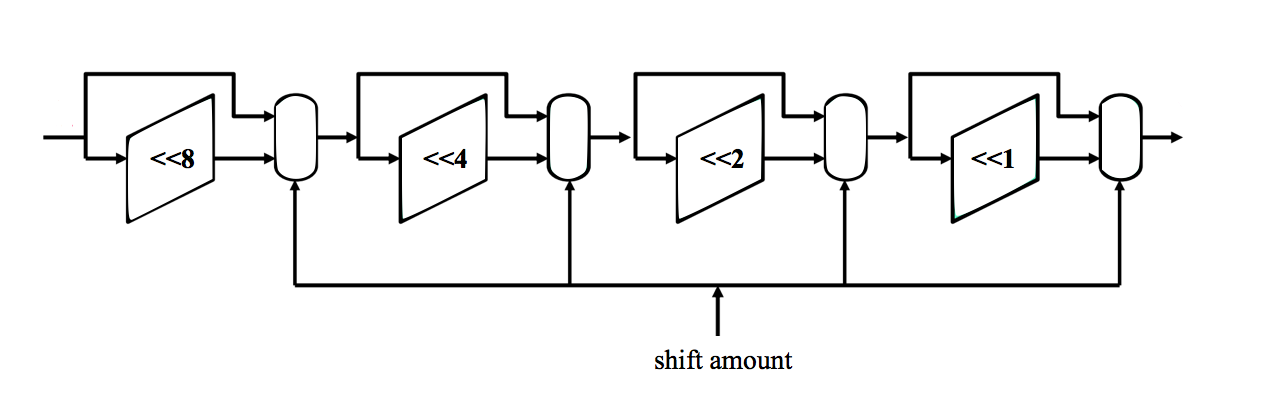
\includegraphics[width=8cm]{Barrelshift.png}
    \caption{Schematic of left logical barrel shifter}
    \label{fig:my_label}
\end{figure}
\paragraph{Left logical shifter:}
A barrel shifter that can shift a value 16, 8, 4, 2, and 1 time(s), or any combination of those. When the input is shifted left, a 0 is put in the least significant bit's place, since it is a logical shift.
\paragraph{Right arithmetic shift:}
A barrel shifter that can shift a value 16, 8, 4, 2, and 1 time(s), or any combination of those. When the input is shifted right, a 0 or 1 is put in the most significant bit's place, based on what the most significant bit of the original data\_operandA is, since it is an arithmetic shift.

\subsubsection{ALU Status Flags}
\paragraph{isNotEqual:} Two operands are not equal if their difference is nonzero. If the OR output of every bit in the adder's output is 1, then we know the 32 bit quantity is nonzero. This was done in the isNotZero module. \newline

\paragraph{isLessThan:} Operand A is strictly less than operand B if their difference produces a negative value. Therefore by checking the most significant bit of the adder module output, one can determine if A<B. One special case occurs when subtraction produces overflow and the most significant bit becomes 0. This was accounted for by an OR gate containing overflow and the most significant bit of the adder's output. \newline

\paragraph{overflow:}
Overflow can be determined by the xor of the most significant bit's carry in and carry out. This was generated in the 32 bit adder and passed to the ALU. 
\newline
\subsubsection{Challenges Faced when Implementing ALU}
When submitted, the ALU was too slow for a handful of testbench cases. The adder was the primary cause of this. The two tests that failed in time trials were the longest latency commands that can occur: subtracting 0 from 0 yielded incomplete results, and isNotEqual was incorrectly set for 0-0. For subtracting 0 minus 0, all of the B operand bits must be converted to 1, XOred with the A input, added together (with a carry in every case). To set the isNotEqual flag, an addition operation must complete and then each of the adder's output bits must be or'ed to determine if the answer is zero. In this test case, 0 is also subtracted from zero. \newline
This bug was solved before using the adder in multdiv. It was solved by adding a submodule that checks whether both of the ALU input operands are zero, and automatically sends zero to the ALU output and sets isNotEqual to 0. This allowed for the bypassing of the slow adder circuitry.

\subsection{Multdiv}
The multdiv module is a signed 32-bit integer multiplier and divider unit. The module handles signed integers in two’s complement, and asserts a data\_exception on overflow or division by 0. When a multiplication or division operation is complete, the data\_resultRDY signal is produced.
A multiplication or division operation begins when the ctrl\_MULT and ctrl\_DIV go high. Since these signals are only high for one clock cycle, they are stored in 1 bit dflipflops to determine whether the division module or multiplication module output should be output from the multdiv unit. The reassertion of a ctrl\_MULT or ctrl\_DIV, or the assert of data\_resultRDY, resets the the multiplication and division modules. More specific details about the implementation of each operation and overflow checking can be found below.

\subsubsection{Multiplication (see Figure 2)}
Multiplication was implemented using modified Booth's algorithm. It takes 16 clock cycles to complete. \newline 
When ctrl\_MULT is asserted, the multiplier input is fed to a control module which outputs 3, 16-bit vectors that specify what clock cycles require a shifted multiplicand, a subtraction operation, or nothing to be done. A vector bit is read based on which bit of the 16 bit counter is high. \newline
In parallel to the Booth control module, the input multiplicand and the input multiplicand shifted left by 1 are fed into a mux. The shift flag from the booth control determines which of these two inputs is fed into a mini\_ALU. The mini\_ALU can perform three operations: add, subtract, or pass an input to the output. The opcode for this ALU is determined by the subtract and nothing bits produced in the control module earlier. It is unnecessary to generate -M and -2M required for modified Booth's beforehand because if subtraction is asserted in the mini\_ALU, the generation of -M and -2M will occur internally. This design decision was made with the knowledge that the subtraction operation is guaranteed to occur in less than one clock cycle, and there is no other high latency step in mult.\newline
The output of the mini\_ALU is then fed into the top 32 bits of a 64 bit  register which shifts any input fed to it right by 2. The result of the multiplication is ready when the 16th bit of the counter is high.
\paragraph{Multiplication Overflow:}
Overflow is checked for in every addition operation in multiplication. The final result of the multiplication is also checked for sign overflow. A particular edge case that was considered was multiplying the largest positive number by itself.
\newline
\begin{figure}[h]
    \centering
    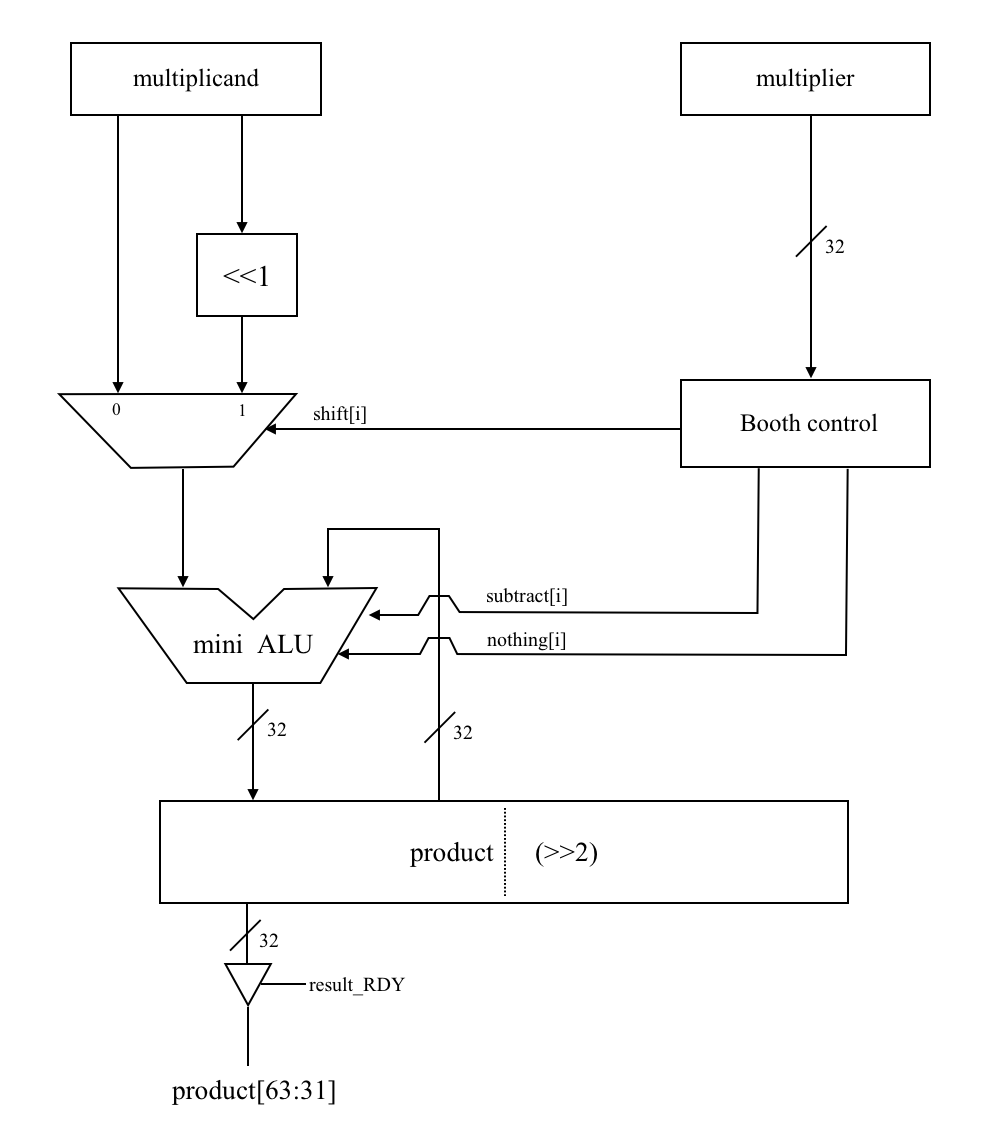
\includegraphics[width=8cm]{Multiply.png}
    \caption{Overview of Multiplication Circuit}
    \label{fig:my_label}
\end{figure}

\subsubsection{Division (see Figure 3)}
Division was implemented using a closed loop in hardware. A division operation takes 34 cycles. First, the dividend is fed into the lower 32 bits of a 64 bit register that shifts inputs left by 1. On every subsequent cycle, the divisor is subtracted from the top 32 bits of the 64 bit shifting register. If the remainder is greater than or equal to 0, the top 32 bits of the 64 bit register are written and a 1 is written to the least significant bit. Otherwise, the previous remainder is written back to the register. \newline
An important design decision that was made was how to deal with negative numbers. Only positive operands are fed to the add/subtract module. On every assertion of ctrl\_DIV, the 2s complement of both operands is found, and used as the divider/dividend if the input is originally negative. If only one of the operands is negative, the output is inverted at the end. Unfortunately, this inverting adds two clock cycles to my division and is very hardware intensive: finding the 2s complement of the input operands and the output requires instantiating three additional adders to add 1 to inverted operands; an addition operation is guaranteed to complete in one clock cycle, therefore an extra clock cycle is required at the beginning and end of the division operation. 

\paragraph{Division Overflow:}
Overflow only possible when dividing by zero. Therefore, every bit of the divisor is or-ed with each other to determine if it is nonzero.
\newline
\subsubsection{Challenges Faced when Implementing Multdiv}
Multiplication and division were designed as closed loops in hardware. The most challenging aspect of creating this loop was timing. It was difficult to create and coordinate counters that fed correct control bits at the correct cycle.
\begin{figure}[h]
    \centering
    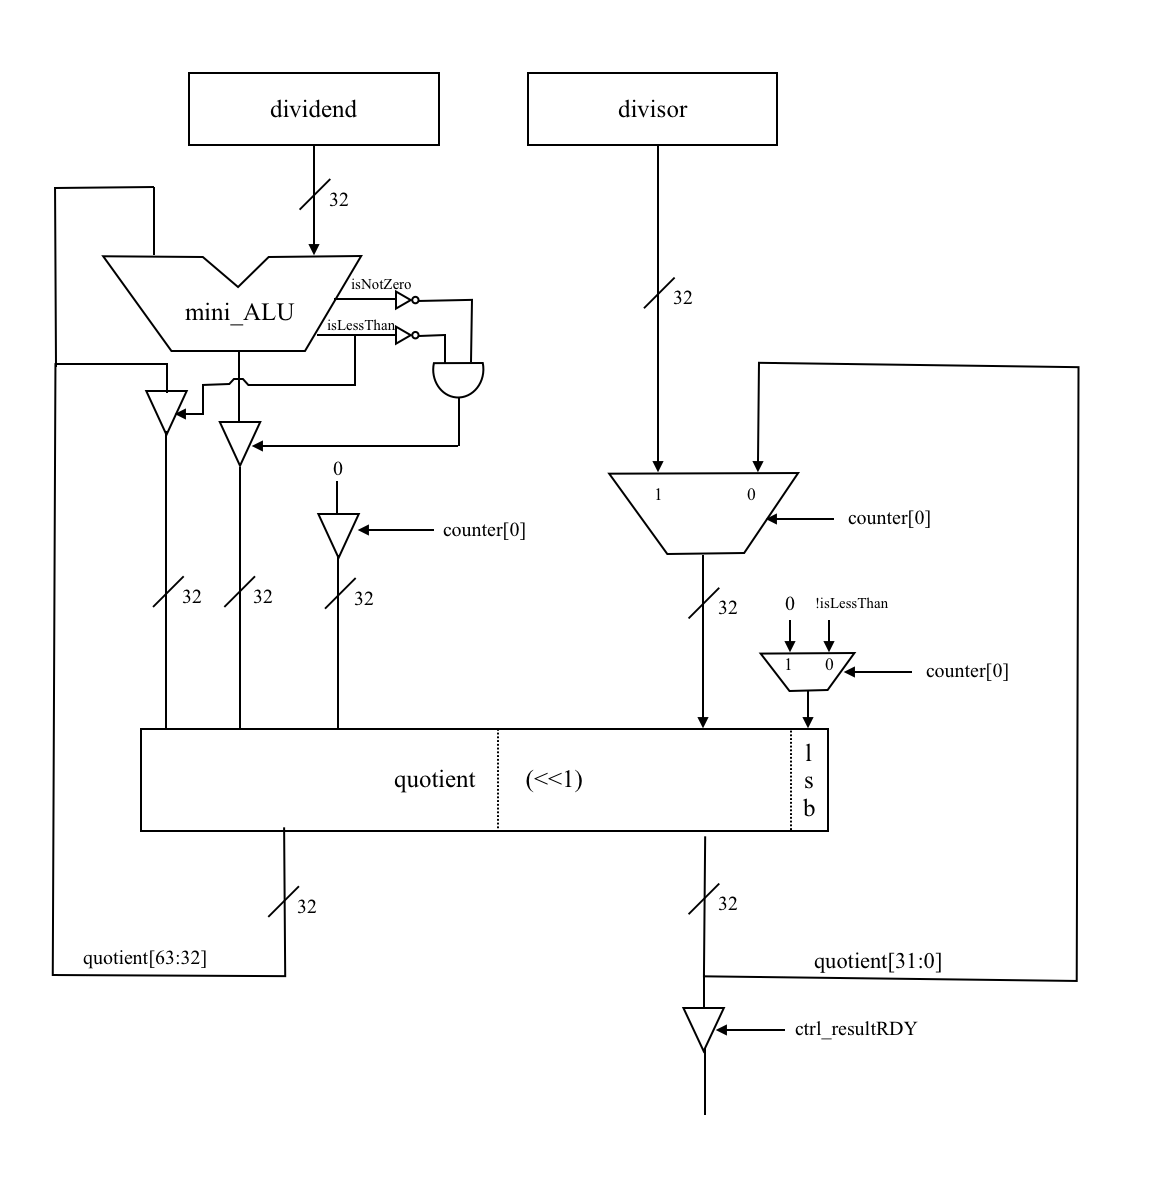
\includegraphics[width=\textwidth]{Divide.png}
    \caption{Overview of Division Circuit}
    \label{fig:my_label}
\end{figure}
\clearpage
\section{Full Processor}
The implementation of a 5 stage pipelined processor closely followed the implementation of the pipelined processor discussed in class. Any significant deviations from the pipeline design shown in lecture are justified in the appropriate stage. An important design feature of the pipeline is that the multdiv module runs outside of the 5 stage pipeline, please see the "Multdiv in the pipeline" subsection. 

\subsection{Memory Elements}
\subsubsection{Register file}
Instance of regfile module described earlier. Important register conventions of this pipeline include:
\begin{enumerate}
    \item \$r0 always reads 0
    \item \$r30 is the status register
    \item \$r31 is the return address register
\end{enumerate}
Both \$r30 and \$r31 can be set and overwritten by any instruction. However, precedence is given to writing exception codes to \$r30.
\subsubsection{imem}
Single port ROM generated from the Altera IP catalog. \newline
\textbf{Inputs:} 12 bit address, clock \newline
\textbf{Output:} 32 bit instruction
\subsubsection{dmem}
Single port RAM generated from the Altera IP catalog. \newline
\textbf{Inputs:} 12 bit address, clock, write enable control \newline
\textbf{Output:} 32 bit instruction

\subsection{F stage (see Figure 4)}
Overview of actions take in this stage:
\begin{enumerate}
    \item storage and computation of next PC (deciding whether to write PC+1 or a branch's jump address to the PC register)
    \item fetch an instruction from ROM memory based on current PC
\end{enumerate}
\begin{figure}[h]
    \centering
    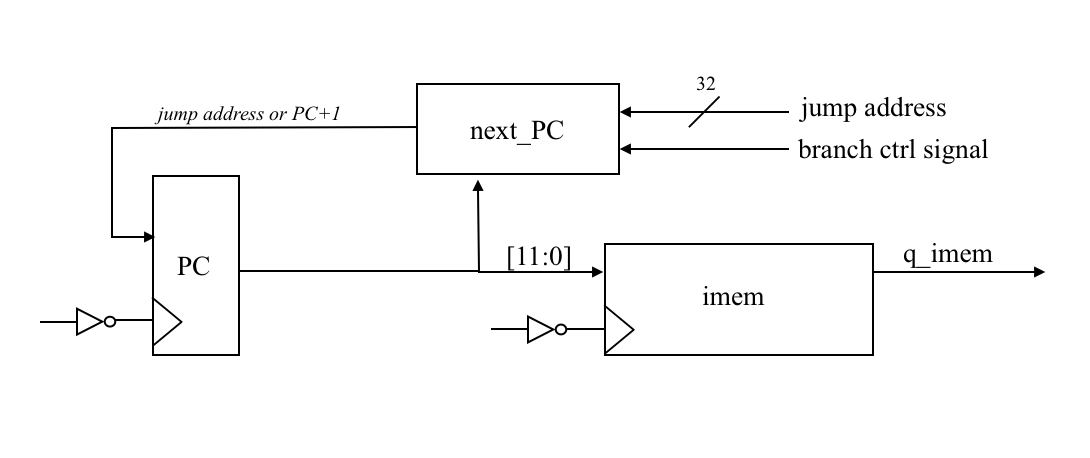
\includegraphics[width=\textwidth]{Fetch.png}
    \caption{Overview of Fetch Stage}
    \label{fig:my_label}
\end{figure}

\subsection{D stage (see Figure 5)}
Actions take in this stage:
\begin{enumerate}
    \item decoding of instruction type
    \item retrieving data from register file
    \item sign extending immediate 
    \item inserting nop in case of stall
    \item if multiplication, load operands to multdiv unit
    \item if stall, nop written to DX register
\end{enumerate}
\paragraph{Justification of 1:} In future pipeline stages, control logic can be implemented effectively using just the type (R, I, JI, JII) of an instruction. Therefore, the instruction type was decoded and then encoded as a two bit value that was propagated through the pipeline registers. This decreased the latency of certain logic generation.
\paragraph{Justification of action 3:} The execute stage is the most hardware intense stage. In order to decrease the latency of generating the inputs required for the ALU in the execute stage, the immediate is sign extended in the F stage and that value is saved in the FD register to potentially be used in the execute stage. 
\paragraph{Justification of action 5:} The multdiv module requires that its operands are stable for the entire multi-cycle process. Therefore, the operands must be written to registers before ctrl\_MULT and ctrl\_DIV are asserted in the execute stage, since multdiv operations begin immediately on their assertion. Therefore, the values of multdiv operands are loaded in the Fetch stage. This design decision requires additional bypassing to be implemented specifically for multdiv instructions.
\paragraph{Justification of action 6:} Follows the MIPS processor delayed branch model.
\begin{figure}[h]
    \centering
    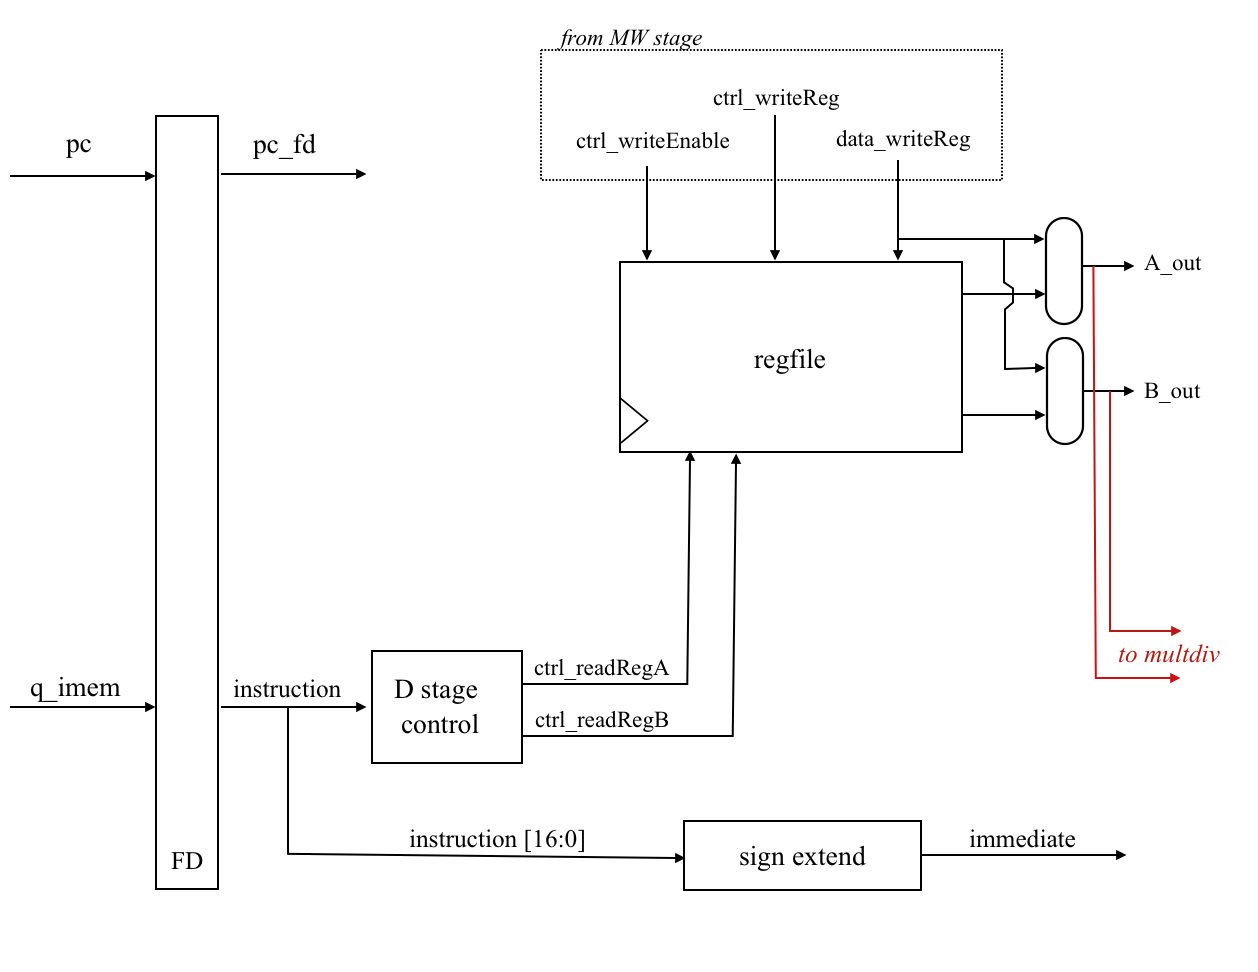
\includegraphics[width=\textwidth]{Decode.png}
    \caption{Overview of Decode Stage}
    \label{fig:my_label}
\end{figure}
\clearpage
\subsection{X stage (see Figure 6)}
Actions take in this stage:
\begin{enumerate}
    \item computations using ALU
    \item branch target address computed
    \item branch taken/not taken resolution
    \item redirection of values in the case of special instructions
\end{enumerate}
\paragraph{Justification of 5:} For certain instructions, the value written to a register is not the ALU output, nor the sign extended immediate, nor the value stored in the second register read. Such instructions, such as jal, setx, and any overflow, must have PC+1, the target, or an exception status, written to a register. 
\begin{figure}[h]
    \centering
    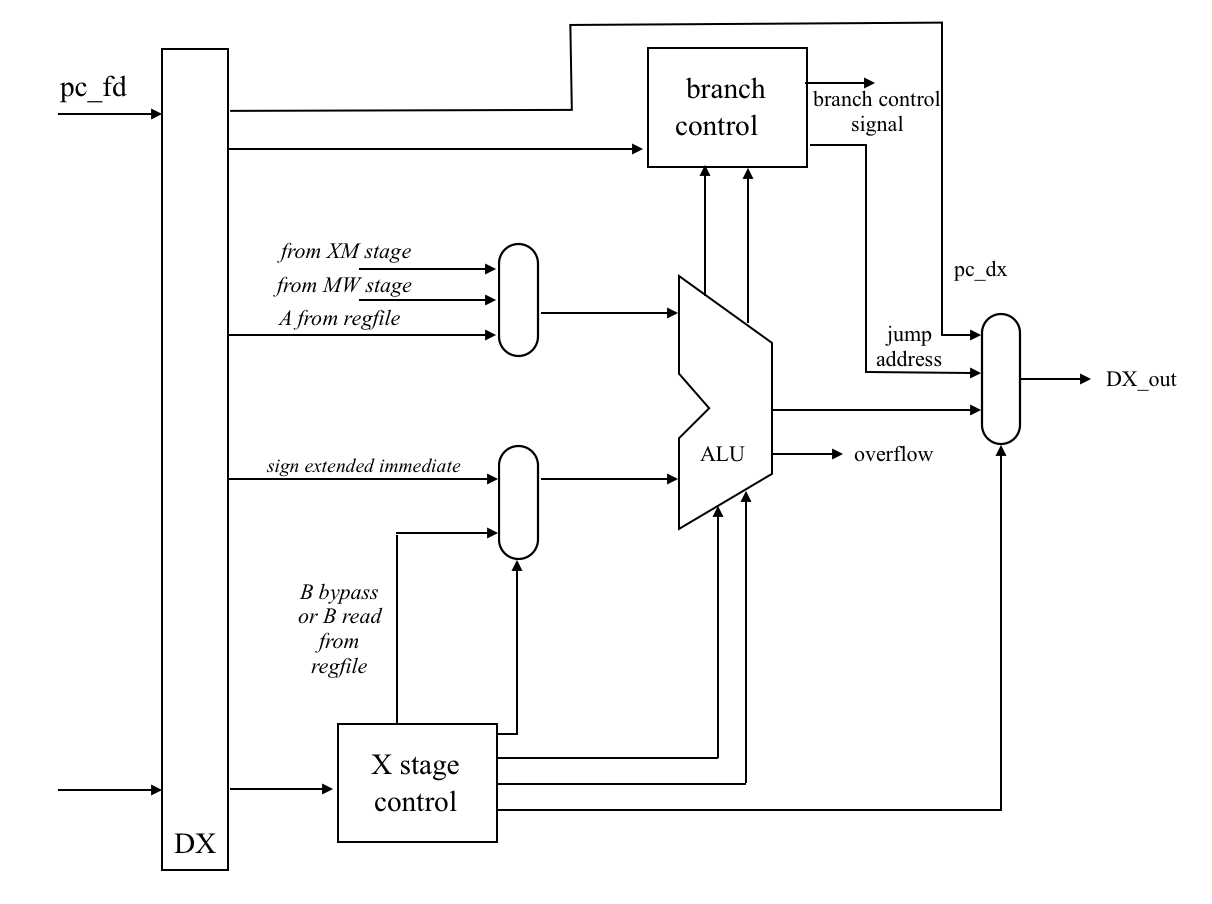
\includegraphics[width=\textwidth]{Execute.png}
    \caption{Overview of Execute Stage}
    \label{fig:my_label}
\end{figure}

\subsection{M stage (see Figure 7)}
Actions take in this stage:
\begin{enumerate}
    \item reading from RAM memory during load word
    \item writing to RAM memory during store word
\end{enumerate}
\begin{figure}[h]
    \centering
    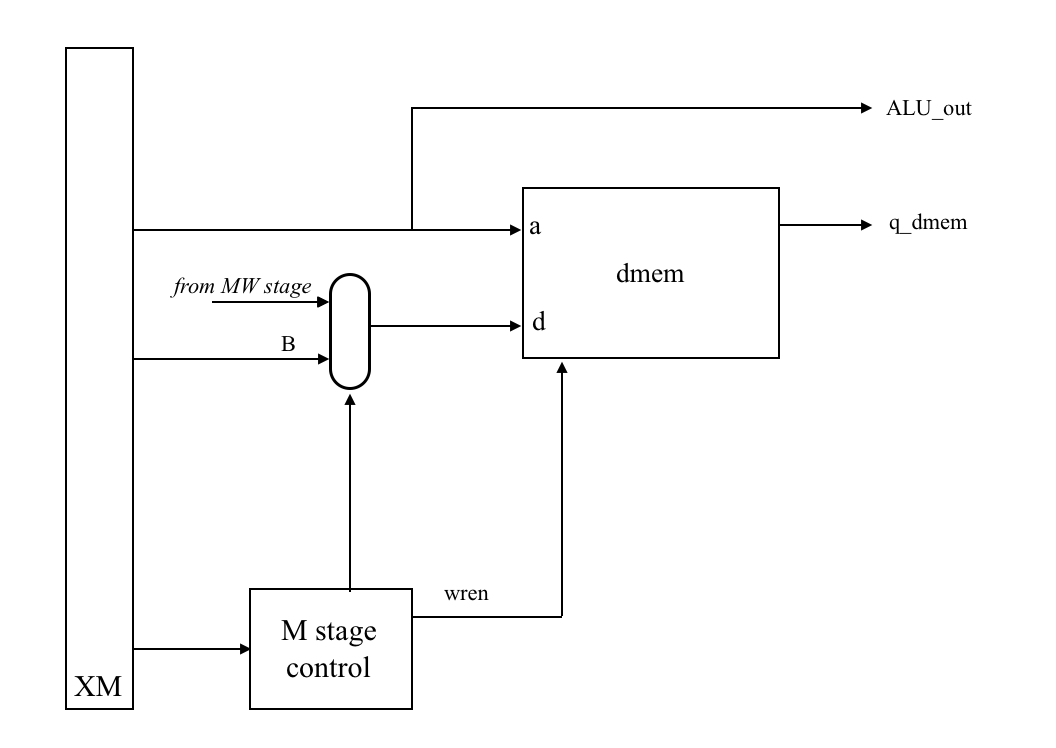
\includegraphics[width=\textwidth]{Memory.png}
    \caption{Overview of Memory Stage}
    \label{fig:my_label}
\end{figure}

\subsection{W stage (see Figure 8)}
Actions take in this stage:
\begin{enumerate}
    \item selecting value to write back to regfile (if any)
    \item selecting register to write (if any)
    \item codifying exceptions by writing to \$rstatus
\end{enumerate}
\begin{figure}[h]
    \centering
    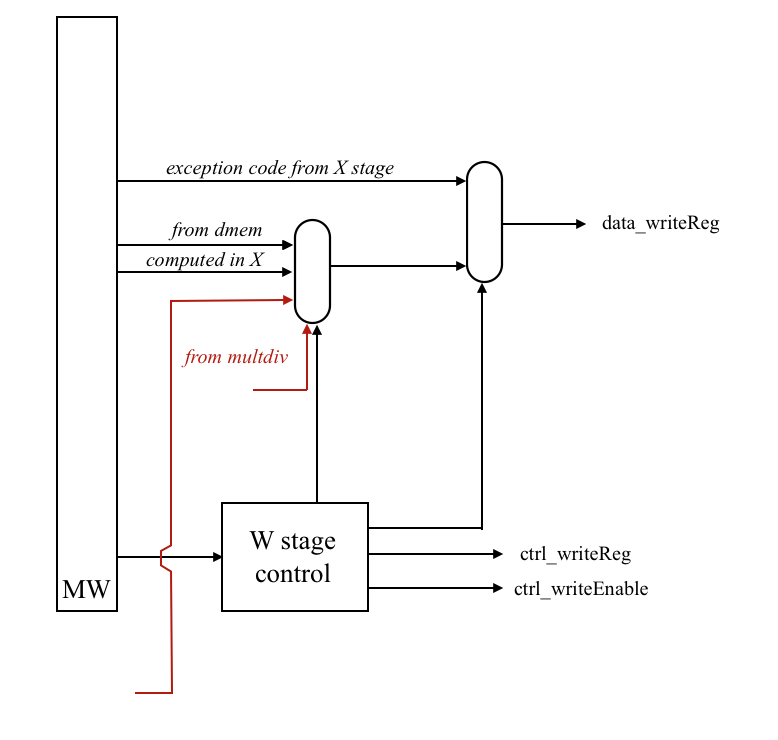
\includegraphics[width=\textwidth]{Write.png}
    \caption{Overview of Write Stage}
    \label{fig:my_label}
\end{figure}
\clearpage
\subsection{Multdiv "in" the pipeline}
\begin{figure}[h]
    \centering
    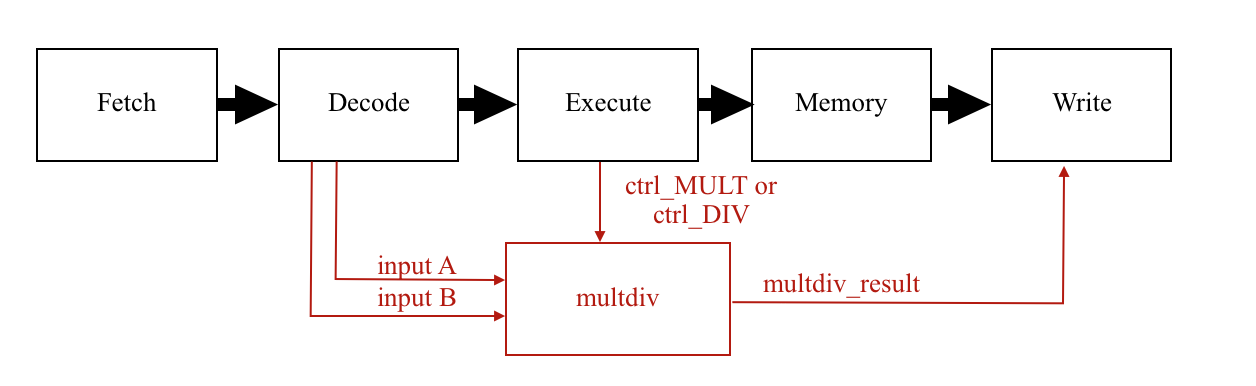
\includegraphics[width=\textwidth]{multdiv.png}
    \caption{Data flow of multiplication and division operation}
    \label{fig:my_label}
\end{figure}
Multdiv is a time consuming, multicycle process. Therefore, it has been placed outside of 5 stage pipeline. Its required operands are routed to the module in the Decode stage, and the multdiv result is written back in the Write stage. Therefore, multdiv operation completely bypass the execute and memory stage. 
Unfortunately, due to this, multdiv operands do not have access to the A and B input bypasses in the execute stage. Due to time constraints, it was not possible to construct the bypasses required for multdiv operands. Therefore \textbf{A known bug in the pipeline} is that multdiv will fail if its sources are registers that will be written by instructions in the execute or memory. 

\subsection{Pipeline Control}
The avoids data and control hazards through stalls and bypasses. 
\subsubsection{Stalls}
The pipeline stalls in two cases:
\begin{enumerate}
    \item data being read from memory is a source in the following instruction
    \item multdiv is in progress
    \item branch is taken
\end{enumerate}
\paragraph{Justification of 2:} Ideally, multdiv would run in parallel to the pipeline and only stall if the source register of a following instruction required the multdiv result as its source. However, due to timing constraints, this was not implemented. Instead, the entire pipeline stalls for the 16 cycle multiplication or 32 cycle division operation.

\subsubsection{Bypassing}
There are 5 bypasses in the processor. Some general logic applied to bypassing is found here:
\begin{enumerate}
    \item If the destination register of an instruction in the the memory or write stage is the source of an instruction in the execute stage, bypass. EXCEPTION: do not bypass if the destination register of an instruction in the the memory or write stage was actually a source (eg bne, blt).
    \item Do not bypass when there is a nop.
    \item Bypass when reading a register being written on the same cycle.
\end{enumerate}
\paragraph{ALU input A \& B bypass (see figure 10):} This bypass occurs when the instruction in the M or W stage is writing to a source register of the instruction in the X stage.
\begin{figure}[h]
    \centering
    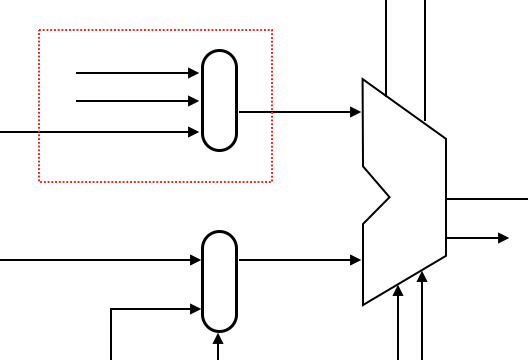
\includegraphics[width=4cm]{ALUinbypass.png}
    \caption{ALU input A bypass in X stage}
    \label{fig:my_label}
\end{figure}

\paragraph{dmem data bypass (see figure 11):} This bypass occurs when the instruction in the W stage is writing to the register being written to memory in the M stage during a store word operation.
\begin{figure}[h]
    \centering
    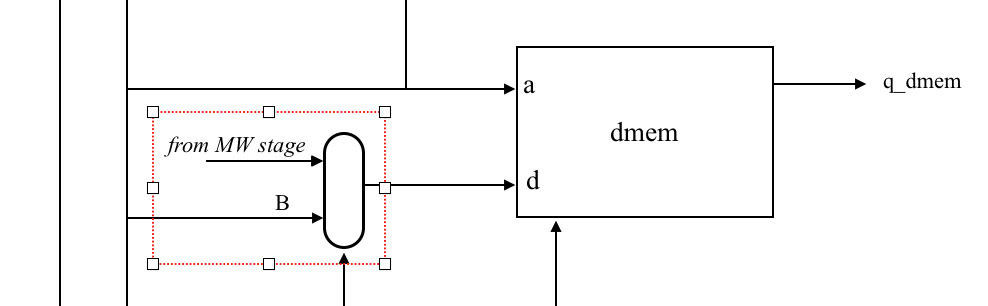
\includegraphics[width=6cm]{dmemdatabypass.png}
    \caption{Dmem data bypass in M stage}
    \label{fig:my_label}
\end{figure}

\paragraph{regfile read A \& B bypass (see figure 12):} Regfile writes on the positive edge of the clock. Therefore, if the instruction in the W stage is writing to a register when an instruction in F stage is reading from that register, the unwritten value will be read.
\begin{figure}[h]
    \centering
    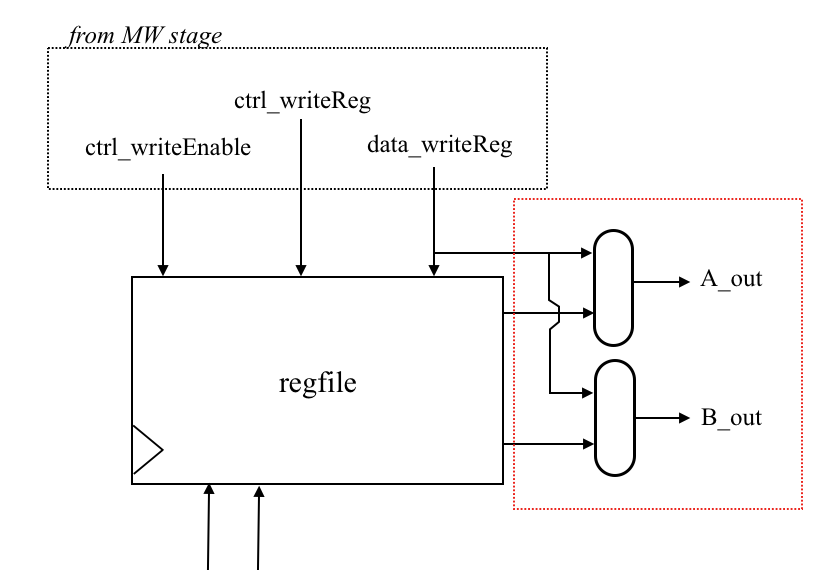
\includegraphics[width=6cm]{regreadbypass.png}
    \caption{Read register bypass in F stage}
    \label{fig:my_label}
\end{figure}

\subsubsection{Branching}
An important set of instructions in the pipeline API involves branching. Branches change the value written to the PC register. There are three different ways a branch instruction may alter the PC:
\begin{enumerate}
    \item PC = extended 26 bit target
    \item PC = PC + 1 + N
    \item PC = value in a register
\end{enumerate}
There is a mini\_ALU module in the branch control that computes type 2 jump addresses. The execute stage ALU cannot be used because in some cases type 2 branch resolution is determined by the relation of two register values to each other (eg bne, blt) which requires computation in the ALU. 
\newline
All jump addresses and branch taken/not taken logic takes place in the execute stage. To avoid control hazards, when a branch is taken, the FD and DX pipeline registers are flushed and a nop is inserted into the DX register.

\subsection{Clocking}
The pipeline operates correctly with a 50 MHz clock. The clocking schema of clocked subcomponents in the processor are described below.
\begin{enumerate}
    \item \textbf{PC register:} write on negative edge
    \item \textbf{imem:} read on negative edge
    \item \textbf{pipeline registers:} write on positive edge
    \item \textbf{regfile:} read/write on positive edge
    \item \textbf{multdiv:} starts operation on positive edge
    \item \textbf{dmem:} read/write on negative edge
\end{enumerate}

\subsection{Efficiency details}
The efficiency of the processor was considered in two ways: chip area efficiency and timing efficiency. Area was optimized for by trying to minimize the size of modules. For example, a modified Booth multiplier was built instead of a Wallace Tree multiplier. Additionally, a pared down ALU is used in parts of the processor that do not require all the functionality of the full ALU. The trade-off for this optimization is an increased amount of time spent computing multiplication and division operations. Timing was optimized for by adding bypass logic to avoid stalling. This latter point is where more optimization could be added. For example, the construction of a branch predictor would increase the time efficiency of the processor by decreasing the number of times one needs to stall and flush after branches. Regardless, the processor clocks at 50MHz during local testing, thus meeting the specified design requirements.

\section{Instruction Implementation}
The processor ISA contains 18 instructions. Below is a  description of how every instruction behaves in the pipeline.
\subsection{add \$rd, \$rs, \$rt}
Operation: \$rd = \$rs + \$rt (\$rstatus = 1 if overflow)
\begin{enumerate}
    \item \textbf{Decode:} \$rs \& \$rt read from regfile or taken from write bypass
    \item \textbf{Execute:} ALU opcode decoded->values of \$rs \& \$rt  fed to ALU->sum is output from X stage; if exception occurs, pass 001 as exception
    \item \textbf{Memory:} no action
    \item \textbf{Write:} destination register decoded->sum written back to regfile; if exception, select \$rstatus as destination register and write exception code
\end{enumerate}

\subsection{addi \$rd, \$rs, N}
Operation: \$rd = \$rs + N
\$rstatus = 2 if overflow
\begin{enumerate}
    \item \textbf{Decode:} \$rs read from regfile or taken from write bypass, 17 bit N immediate sign extended to 32 bits
    \item \textbf{Execute:} ALU opcode set to add operation, sign extended immediate is selected as ALU input B->ALU computes sum->sum output from DX stage; if exception occurs, pass 002 as exception
    \item \textbf{Memory:} no action
    \item \textbf{Write:} destination register decoded->sum written back to regfile; if exception, select \$rstatus as destination register and write exception code
\end{enumerate}

\subsection{sub \$rd, \$rs, \$rt}
Operation: \$rd = \$rs - \$rt (\$rstatus = 3 if overflow)
\begin{enumerate}
    \item \textbf{Decode:} \$rs \& \$rt read from regfile or taken from write bypass
    \item \textbf{Execute:} ALU opcode decoded->values of \$rs \& \$rt  fed to ALU->difference is output from X stage; if exception occurs, pass 003 as exception
    \item \textbf{Memory:} no action
    \item \textbf{Write:} destination register decoded->sum written back to regfile; if exception, select \$rstatus as destination register and write exception code
\end{enumerate}

\subsection{and/or \$rd, \$rs, \$rt}
Operation: \$rd = \$rs \& \$rt / \$rd = \$rs | \$rt
\$rstatus = 2 if overflow
\begin{enumerate}
    \item \textbf{Decode:} \$rs \& \$rt read from regfile or taken from write bypass
    \item \textbf{Execute:} ALU opcode decoded->values of \$rs \& \$rt  fed to ALU->ALU output is output of X stage
    \item \textbf{Memory:} no action
    \item \textbf{Write:} destination register decoded->ALU output written back to regfile
\end{enumerate}

\subsection{sra/sll \$rd, \$rs, shamt}
Operation: \$rd = \$rs << shamt / \$rd = \$rs >>> shamt
\begin{enumerate}
    \item \textbf{Decode:} \$rs read from regfile or taken from write bypass
    \item \textbf{Execute:} ALU opcode \& shift amount decoded from instruction ->values of \$rs \& \$rt  fed to ALU->shift output is output of X stage
    \item \textbf{Memory:} no action
    \item \textbf{Write:} destination register decoded->ALU output written back to regfile
\end{enumerate}

\subsection{mul/div \$rd, \$rs, \$rt}
Please see "Multdiv in the pipeline" for a more detailed description of the implementation of multiplication and division in the pipeline.
Operation: \$rd = \$rs * \$rt (\$rstatus = 4 if overflow) /
\$rd = \$rs / \$rt (\$rstatus = 5 if divide by 0)
\begin{enumerate}
    \item \textbf{Decode:} \$rs \& \$rt read from regfile or taken from write bypass
    \item \textbf{Execute:} ctrl\_MULT/ctrl\_DIV decoded; \$rd decoded and sent to multdiv control module, STALL PIPELINE UNTIL RESULT READY & flush DX register
    \item \textbf{Memory:} no action
    \item \textbf{Write:} when result is ready, written back to regfile using saved destination register, pipeline resumes; if exception, select \$rstatus as destination register and write exception code
\end{enumerate}

\subsection{sw \$rd, N(\$rs)}
Operation: MEM[\$rs + N] = \$rd
\begin{enumerate}
    \item \textbf{Decode:} \$rs and \$rd read from regfile or taken from write bypass (\$rd is routed to ctrl\_readRegB) \& 17 bit N sign extended to 32 bits (saved in DX register)
    \item \textbf{Execute:} ALU opcode set to add operation \& sign extended immediate is selected as ALU input B->ALU computes sum->sum output from DX stage (ALU output is the address where we want to store something in memory)
    \item \textbf{Memory:} assert dmem write enabled, use lower 12 bits of ALU output as dmem address, data written to dmem is value stored in \$rd
    \item \textbf{Write:} no action
\end{enumerate}

\subsection{lw \$rd, N(\$rs)}
Operation: \$rd = MEM[\$rs + N]
\begin{enumerate}
    \item \textbf{Decode:} \$rs read from regfile or taken from write bypass \& 17 bit N sign extended to 32 bits (saved in DX register)
    \item \textbf{Execute:} ALU opcode set to add operation \& sign extended immediate is selected as ALU input B->ALU computes sum->sum output from DX stage (ALU output is the address where we want to get something from memory)
    \item \textbf{Memory:} use lower 12 bits of ALU output as dmem address, save dmem out to MW pipeline register
    \item \textbf{Write:} destination register decoded->memory output written back to regfile
\end{enumerate}

\subsection{j T}
Operation: PC = T
\$rstatus = 2 if overflow
\begin{enumerate}
    \item \textbf{Decode:} no action
    \item \textbf{Execute:} target is extended to 32 bits->set jump address to extended target->assert take\_branch (will write this address as new PC)->signal to insert nop at DX pipeline register & flush FD and DX register
    \item \textbf{Memory:} no action
    \item \textbf{Write:} no action
\end{enumerate}

\subsection{bne \$rd, \$rs, N }
Operation: if (\$rd != \$rs) PC = PC + 1 + N
\begin{enumerate}
    \item \textbf{Decode:} \$rs and \$rd read from regfile or taken from write bypass (\$rd is routed to ctrl\_readRegB) \& 17 bit N sign extended to 32 bits (saved in DX register)
    \item \textbf{Execute (in branch control):} sign extended immediate added to pc stored in DX register (already PC+1), this is the jump address; write this jump address to PC register ONLY IF isNotEqual from ALU is high->IF TAKEN signal to insert nop at DX pipeline register \& flush FD and DX register
    \item \textbf{Execute:} ALU opcode set to subtraction operation->ALU computes difference->isNotEqual ALU status flag sent to branch control
    \item \textbf{Memory:} no action
    \item \textbf{Write:} no action
\end{enumerate}

\subsection{jal T}
Operation: \$r31 = PC + 1, PC = T
\begin{enumerate}
    \item \textbf{Decode:} no action
    \item \textbf{Execute (in branch control):} target is extended to 32 bits->set jump address to extended target->assert take\_branch (will write this address as new PC)
    \item \textbf{Execute:} X stage output mux selects the pc stored in the DX register on this cycle to be saved in XM register
    \item \textbf{Memory:} no action
    \item \textbf{Write:} \$r31 set as destination register->pc written to \$r31
\end{enumerate}

\subsection{jr \$rd}
Operation: PC = \$rd
\begin{enumerate}
    \item \textbf{Decode:} \$rd read from regfile or taken from write bypass (\$rd is routed to ctrl\_readRegB)
    \item \textbf{Execute (in branch control):} rd value is set as jump address -> take\_branch asserted (will write rd value as new PC)
    \item \textbf{Execute:} no action
    \item \textbf{Memory:} no action
    \item \textbf{Write:} no action
\end{enumerate}

\subsection{blt \$rd, \$rs, N }
Operation: if (\$rd < \$rs) PC = PC + 1 + N
\begin{enumerate}
    \item \textbf{Decode:} \$rs and \$rd read from regfile or taken from write bypass (\$rd is routed to ctrl\_readRegB) \& 17 bit N sign extended to 32 bits (saved in DX register)
    \item \textbf{Execute (in branch control):} sign extended immediate added to pc stored in DX register (already PC+1), this is the jump address; write this jump address to PC register ONLY IF ~isLessThan (since \$rd is input B to ALU) from ALU is high->IF TAKEN signal to insert nop at DX pipeline register \& flush FD and DX register
    \item \textbf{Execute:} ALU opcode set to subtraction operation->ALU computes difference->isLessThan ALU status flag sent to branch control
    \item \textbf{Memory:} no action
    \item \textbf{Write:} no action
\end{enumerate}

\subsection{bex T}
Operation: IF (\$rstatus != 0) PC = T
\begin{enumerate}
    \item \textbf{Decode:} ctrl\_readRegB set to \$r30
    \item \textbf{Execute (in branch control):} target is extended to 32 bits->set jump address to extended target & value read from \$r30 is zero by or-ing every bit in value->if nonzero, assert take\_branch (will write extended target as new PC)
    \item \textbf{Memory:} no action
    \item \textbf{Write:} no action
\end{enumerate}

\subsection{setx T}
Operation: \$rstatus = T
\begin{enumerate}
    \item \textbf{Decode:} no action
    \item \textbf{Execute (in branch control):} target is extended to 32 bits
     \item \textbf{Execute:} extended target from branch control is selected as the output of the DX stage instead of ALU or PC
    \item \textbf{Memory:} no action
    \item \textbf{Write:} destination register is set to \$r30 and extended target is written back to regfile
\end{enumerate}

\section{Process}
\subsection{General Implementation Overview}
For previous project checkpoints, I incrementally tested every module I built before putting together the final product. I did not take this approach when building my processor. Instead, I immediately strung together all the processor components, and then went back to debug before implementing bypassing, branching, and multdiv. I found this approach better because I knew how the pipeline was supposed to behave from end to end, so debugging was a matter of narrowing down where an inter-connectivity issue was coming from. I implemented components of my processor in the following order:
\begin{enumerate}
    \item creating 5 stage pipeline with latches
    \item fiddle with clocking schemas for imem, dmem, pc register, and regfile until it worked as expected
    \item add in bypassing & stalling based on lecture slides (ALU inputs and destination)
    \item realize clocking schema requires another bypass in decode stage
    \item implement branching
    \item integrate multdiv
\end{enumerate}

\subsection{Testing Methodology}
When the processor was constructed, I began writing simple MIPS programs to test it on. I wrote a program that tested one specific instruction of feature of the pipeline, and then wrote out where the programmer expects data to be and when in comments. If my processor did not behave as expected, I was able to more clearly trace where things were going wrong, because I knew what values were supposed to exist and when.

\subsection{Learning Points}
\begin{enumerate}
    \item It's 10\% coding, 90\% debugging.
    \item Drawing it out really does help.
    \item It's more complicated than the way we did it in 250.
    \item It's not going to be perfect the first time around, and iterating on a design is a good thing.
\end{enumerate}
\subsection{Challenges}
\begin{enumerate}
    \item Time. In two ways. One, getting my designs to work on a 50MHz clock was always the most difficult part. Twice I had to completely rewrite and implementation because it worked fine unlocked, and completely failed when clocked. Second, time in the real world to complete the assignments.
    \item Mismatch of lecture material covered and project checkpoint requirements. I found it challenging to start early on project checkpoints when material about the checkpoint hadn't been covered in class. For example, for the ALU checkpoint, I started early and implemented a ripple carry adder, only to learn in lecture two days later that that was not fast enough.
\end{enumerate}

\section{Conclusion}
To conclude, I have constructed every part of a five-stage, single-issue, 32-bit processor in structural Verilog. There are still bugs (see Appendix A) and many inefficiencies with the design, however, it's functional.

\clearpage

\section{Appendix A: Known Bugs}
\begin{enumerate}
    \item If multdiv operands needs to be bypassed from the execute or memory stage, multdiv output will be wrong. This is because there is not stall of bypass logic to account for this situation in multdiv. This has been explained previously in "Multdiv in the pipeline." See code example and waveform output in figure .
    \item Bypassing an \$rstatus exception value doesn't work. This is because the bypass logic does not account for an \$rd that cannot be decoded from an instruction, or isn't a jal. See code example and waveform output in figure .
\end{enumerate}

\begin{figure}[h]
    \centering
    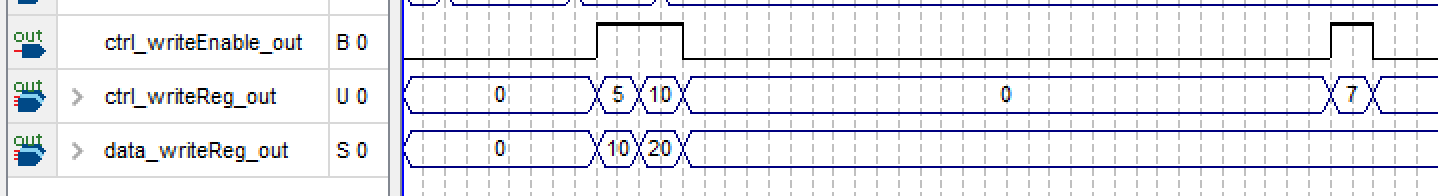
\includegraphics[width=\textwidth]{multdivnobypass.png}
    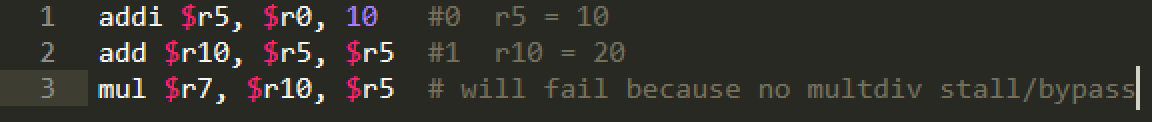
\includegraphics[width=\textwidth]{multdivnobypass_code.png}
    \caption{Code example and waveform output of known bug 1}
    \label{fig:my_label}
\end{figure}

\begin{figure}[h]
    \centering
    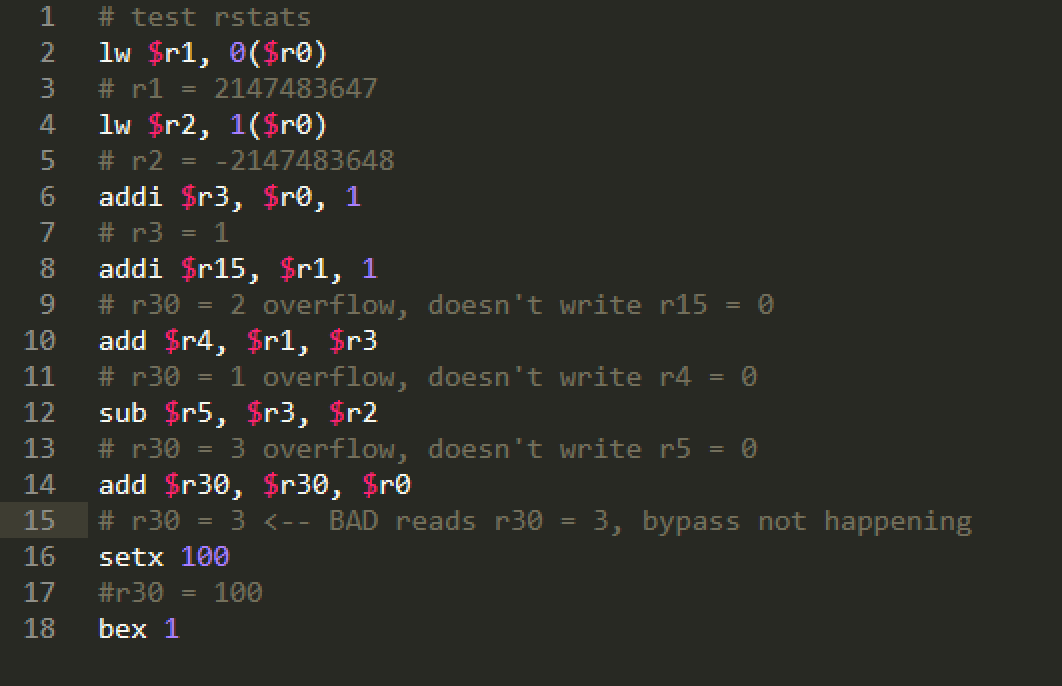
\includegraphics[width=\textwidth]{nobypassrstatus.png}
    \caption{Code example of known bug 2}
    \label{fig:my_label}
\end{figure}

\end{document}
